\documentclass{beamer}

\usepackage[spanish,es-ucroman]{babel}

% Copyright 2017 Sergei Tikhomirov, MIT License
% https://github.com/s-tikhomirov/solidity-latex-highlighting/

\usepackage{listings, xcolor}

\definecolor{verylightgray}{rgb}{.97,.97,.97}

\lstdefinelanguage{Solidity}{
	keywords=[1]{anonymous, assembly, assert, balance, break, call, callcode, case, catch, class, constant, continue, constructor, contract, debugger, default, delegatecall, delete, do, else, emit, event, experimental, export, external, false, finally, for, function, gas, if, implements, import, in, indexed, instanceof, interface, internal, is, length, library, log0, log1, log2, log3, log4, memory, modifier, new, payable, pragma, private, protected, public, pure, push, require, return, returns, revert, selfdestruct, send, solidity, storage, struct, suicide, super, switch, then, this, throw, transfer, true, try, typeof, using, value, view, while, with, addmod, ecrecover, keccak256, mulmod, ripemd160, sha256, sha3}, % generic keywords including crypto operations
	keywordstyle=[1]\color{blue}\bfseries,
	keywords=[2]{address, bool, byte, bytes, bytes1, bytes2, bytes3, bytes4, bytes5, bytes6, bytes7, bytes8, bytes9, bytes10, bytes11, bytes12, bytes13, bytes14, bytes15, bytes16, bytes17, bytes18, bytes19, bytes20, bytes21, bytes22, bytes23, bytes24, bytes25, bytes26, bytes27, bytes28, bytes29, bytes30, bytes31, bytes32, enum, int, int8, int16, int24, int32, int40, int48, int56, int64, int72, int80, int88, int96, int104, int112, int120, int128, int136, int144, int152, int160, int168, int176, int184, int192, int200, int208, int216, int224, int232, int240, int248, int256, mapping, string, uint, uint8, uint16, uint24, uint32, uint40, uint48, uint56, uint64, uint72, uint80, uint88, uint96, uint104, uint112, uint120, uint128, uint136, uint144, uint152, uint160, uint168, uint176, uint184, uint192, uint200, uint208, uint216, uint224, uint232, uint240, uint248, uint256, var, void, ether, finney, szabo, wei, days, hours, minutes, seconds, weeks, years},	% types; money and time units
	keywordstyle=[2]\color{teal}\bfseries,
	keywords=[3]{block, blockhash, coinbase, difficulty, gaslimit, number, timestamp, msg, data, gas, sender, sig, value, now, tx, gasprice, origin},	% environment variables
	keywordstyle=[3]\color{violet}\bfseries,
	identifierstyle=\color{black},
	sensitive=false,
	comment=[l]{//},
	morecomment=[s]{/*}{*/},
	commentstyle=\color{gray}\ttfamily,
	stringstyle=\color{red}\ttfamily,
	morestring=[b]',
	morestring=[b]"
}

\lstset{
	language=Solidity,
	backgroundcolor=\color{verylightgray},
	extendedchars=true,
	basicstyle=\footnotesize\ttfamily,
	showstringspaces=false,
	showspaces=false,
	numbers=none,
	numberstyle=\footnotesize,
	numbersep=9pt,
	tabsize=4,
	breaklines=true,
	showtabs=false,
	captionpos=b
}


\usetheme{default}

\title{Sistema de Votaci\'on Representativa sobre \textit{Quorum}}
\subtitle{Predefensa}
\author{Andy Ledesma Garc\'ia}
\institute{Universidad de La Habana}
\date{\today}

\begin{document}

\begin{frame}
    \titlepage
\end{frame}

\begin{frame}[fragile]
    \frametitle{API del Contrato}
    \framesubtitle{Interfaz P\'ublica}

    \begin{lstlisting}[language=Solidity]
function voteFor(address chosenCandidate) 
    onlyIfVoterAddressRegistered(msg.sender)
    onlyIfVoterAddressRegistered(chosenCandidate) 

function countVotes() 
    view 
    returns (uint[] memory count) 

function getWinnerAddress() view returns (address) 

function getWinnerId() public view returns (uint32)   
    \end{lstlisting}

\end{frame}

\begin{frame}[fragile]
    \frametitle{API del Contrato}
    \framesubtitle{Interfaz del Due\~no}

    \begin{lstlisting}[language=Solidity]
constructor(address[] memory voters) 

function voteFromVoterIdToVoterId(
    uint32 voterId, 
    uint32 chosenCandidateId
) 

function destroy()
    \end{lstlisting}

\end{frame}

\begin{frame}
    \frametitle{Ejemplo}
    \framesubtitle{13 Votantes, 2 Ciclos y 1 Cadena}

    \begin{figure}
        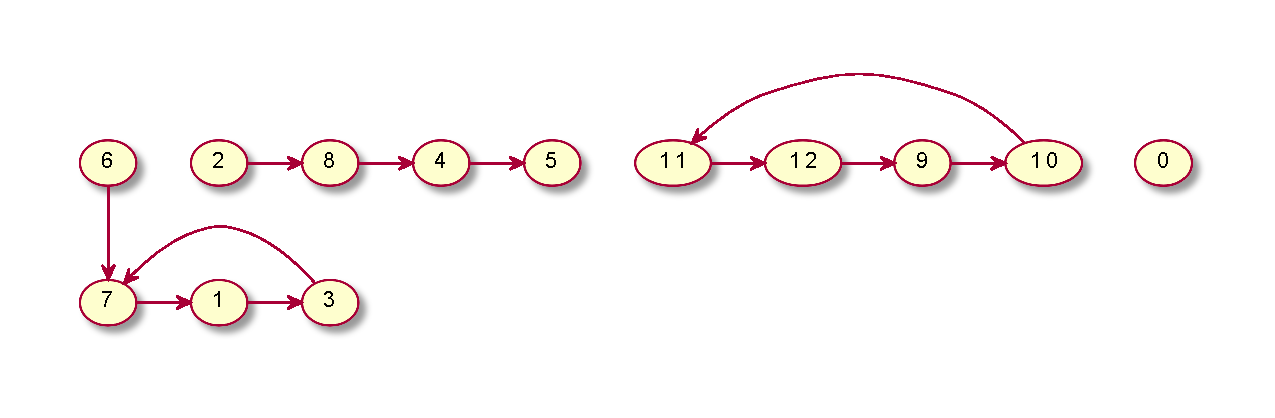
\includegraphics[scale=.5]{graphics/example.pdf}
        \centering
    \end{figure}

    \begin{center}
        \begin{tabular}{r|l}
            Conteo & \\
            0 & 0, 2, 6  \\  
            1 & 8        \\   
            2 & 4        \\   
            3 & 1, 3, 5, 7, 9, 10, 11, 12  
        \end{tabular}
    \end{center}
\end{frame}

\begin{frame}
    \frametitle{Ejemplo}
    \framesubtitle{13 Votantes, 2 Ciclos y 1 Cadena}

    \begin{figure}
        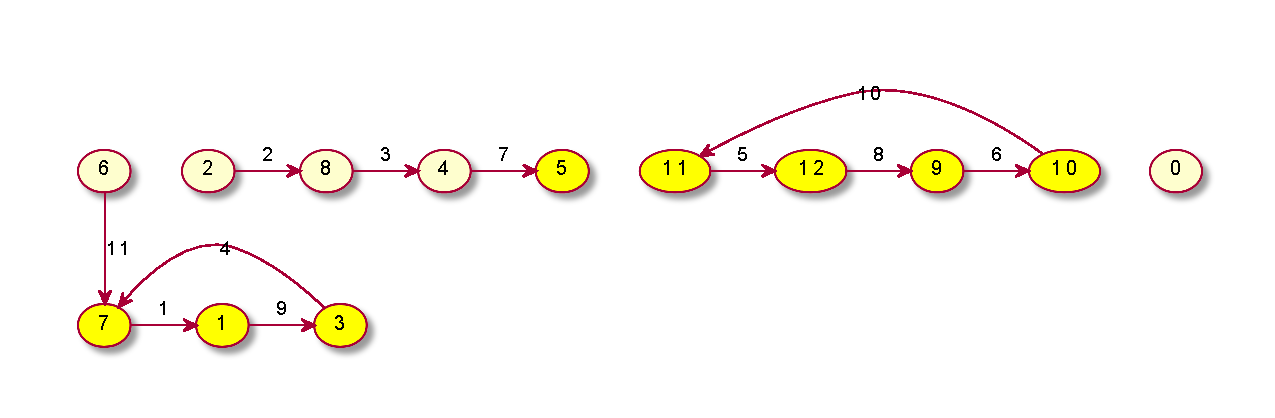
\includegraphics[scale=.5]{graphics/example-tied-colored.pdf}
        \centering
    \end{figure}

    \only<1>{
    \begin{center}
        ronda: 1 $\quad$ mayor\'ia: 6
    \end{center}
    \begin{table}
        \begin{tabular}{|c|c|c|c|c|c|c|c|c|c|c|c|c|c|} \hline
            lugar & 0  & 1  & 2  & 3  & 4  & 5  & 6  & 7  & 8  & 9  & 10 & 11 & 12 \\ \hline                  
            1 &   & 3  & 5  & 7  & 5  &   & 7  & 1  & 5  & 10 & \color{red} 11 & 12 & 9 \\ \hline
            2 &   & 7  &   & 1  &   &   & 1  & 3  &   & \color{red} 11 & 12 & 9 & 10 \\ \hline
            3 &   &    &   &    &   &   & 3  &    &   & 12 & 9 & 10 & \color{red} 11 \\ \hline \hline
            votos &   & 1  &   & 1  &   & 3  &    & 2  &   & 1 & 1 & 1 & 1 \\ \hline
            tiempo &   & 1  &   & 9  &   & 7  &    & 11  &   & 8 & 6 & 10 & 5 \\ \hline
        \end{tabular}
    \end{table}
    }

    \only<2>{
    \begin{center}
        ronda: 2 $\quad$ mayor\'ia: 6
    \end{center}
    \begin{table}
        \begin{tabular}{|c|c|c|c|c|c|c|c|c|c|c|c|c|c|} \hline
            lugar & 0  & 1  & 2  & 3  & 4  & 5  & 6  & 7  & 8  & 9  & 10 & 11 & 12 \\ \hline                  
            1 &   & \color{red} 3  & 5  & 7  & 5  &   & 7  & 1  & 5  & 10 & 12 & 12 & 9 \\ \hline
            2 &   & 7  &   & 1  &   &   & 1  & 3  &   & 12 & 9 & 9 & 10 \\ \hline
            3 &   &    &   &    &   &   & 3  &    &   &    &   & 10 &    \\ \hline \hline
            votos &   & 1  &   & 1  &   & 3  &    & 2  &   & 1 & 1 &   & 2 \\ \hline
            tiempo &   & 1  &   & 9  &   & 7  &    & 11  &   & 8 & 6 & 10 & 10 \\ \hline
        \end{tabular}
    \end{table}
    }

    \only<3>{
    \begin{center}
        ronda: 3 $\quad$ mayor\'ia: 6
    \end{center}
    \begin{table}
        \begin{tabular}{|c|c|c|c|c|c|c|c|c|c|c|c|c|c|} \hline
            lugar & 0  & 1  & 2  & 3  & 4  & 5  & 6  & 7  & 8  & 9  & 10 & 11 & 12 \\ \hline                  
            1 &   & 7  & 5  & 7  & 5  &   & 7  & 1  & 5  & 10 & 12 & 12 & \color{red} 9 \\ \hline
            2 &   &   &   & 1  &   &   & 1  & 3  &   & 12 & \color{red} 9 & \color{red} 9 & 10 \\ \hline
            3 &   &    &   &    &   &   & 3  &    &   &    &   & 10 &    \\ \hline \hline
            votos &   & 1  &   &  &   & 3  &    & 3  &   & 1 & 1 &   & 2 \\ \hline
            tiempo &   & 1  &   &   &   & 7  &    & 11  &   & 8 & 6 & 10 & 10 \\ \hline
        \end{tabular}
    \end{table}
    }

    \only<4-5>{
        \begin{center}
            un tiempo despu\'es...
            
            (me cans\'e de hacer tablas XD)
        \end{center}
    }
    \only<5>{
        \begin{center}
            \textbf{GANA EL 5}
        \end{center}
    }
\end{frame}

\end{document}